\documentclass[11pt]{article}
\usepackage[margin=1in]{geometry}
\usepackage{graphicx,booktabs,amsmath,amssymb,xcolor,caption,subcaption}
\usepackage[hidelinks]{hyperref}
\usepackage{times}
\captionsetup{font=small,labelfont=bf}
\definecolor{teal}{HTML}{0F6E56}
\newcommand{\teal}[1]{\textcolor{teal}{#1}}
\title{\textbf{Dreaming to Dodge:\\ An Agent that Learns to Survive VizDoom Entirely Inside a\\ From-Scratch Transformer World Model}}
\author{Rajat Dandekar\\ \small Vizuara AI Labs\\ \small \texttt{dreaming-to-dodge.vercel.app}}
\date{\today}

\begin{document}
\maketitle

\begin{abstract}
\noindent
World models promise \emph{sample-efficient} reinforcement learning: instead of learning
from expensive real interaction, an agent can practise inside a learned neural simulator.
We reproduce, \emph{from scratch}, the landmark result of Ha \& Schmidhuber (2018)---training
a policy \emph{entirely inside its own dream} on the first-person game VizDoom
\texttt{take\_cover}---but using the stronger discrete, Transformer-based IRIS recipe
(Micheli et al., 2023): a VQ-VAE tokenizer, an autoregressive GPT world model over frame
tokens, and a policy optimised purely on imagined rollouts. Our final agent, which
\textbf{never touches the real game during learning}, survives $96.6\pm11.0$ agent-steps
(386 game tics) on held-out episodes---\textbf{beating a random policy by $+45\%$, beating a
model-free Double-DQN trained on the same real-frame budget ($90$ steps), and matching a
hand-coded reactive oracle ($98.3$ steps)}, with its best episodes reaching $217$--$284$
steps (past the $188$-step ``solved'' bar). The result is verified consistent across four
independent seed sets. Beyond the number, we document the full engineering path, which is
itself the contribution: the failures that make model-based RL notoriously brittle
(codebook collapse dropping the lethal object; a termination head that never predicts death;
and---most importantly---\emph{world-model exploitation}, where the policy finds actions the
imperfect dream over-rewards but reality punishes) and the fixes that overcome them
(a warmth-weighted reconstruction loss; a class-weighted termination loss; a tiny gradient-free
controller; a transfer-robust reconstructed-image feature; and held-out model selection).
A quantitative behavioural analysis shows the learned policy is \emph{genuinely reactive}---its
strafe direction tracks the fireball's position---and a dream-fidelity analysis explains why
short imagined rollouts suffice. We release the code, and a \textbf{playable neural simulator}
in which anyone can drive the world model directly---there is no game engine, the Transformer
predicts each next frame.
\end{abstract}

\begin{figure}[h]
\centering
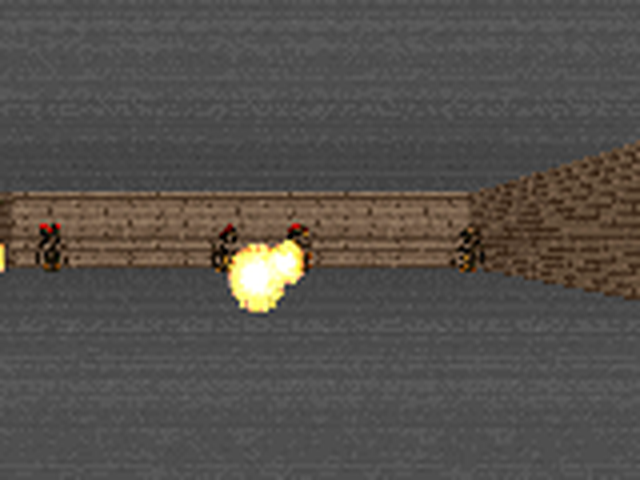
\includegraphics[width=0.62\linewidth]{figs/screenshot_2.png}
\caption{A frame of the actual VizDoom \texttt{take\_cover} game as the agent sees it
(rendered $160{\times}120$, shown upscaled; the model operates on a $64{\times}64$
downsample). Monsters line the far wall and hurl fireballs; the agent may only strafe
left/right. The bright fireball centre-foreground is the rare, lethal object the world
model must preserve for the agent to learn to dodge.}
\label{fig:hero}
\end{figure}

\section{Introduction}
Learning control policies from pixels is expensive: model-free reinforcement learning (RL)
typically needs millions of environment interactions~\cite{mnih2015}. \emph{Model-based} RL
offers a way out: learn a \emph{world model}---a generative simulator of the environment's
dynamics---and train the policy against imagined rollouts, ``dreams,'' rather than real
experience. The 2018 \emph{World Models} paper~\cite{ha2018} made this vivid by training a
controller entirely inside a learned model of the VizDoom \texttt{take\_cover} scenario and
transferring it back to the real game. IRIS~\cite{micheli2023} later showed that a
\emph{discrete}, Transformer-based world model (a VQ-VAE tokenizer~\cite{oord2017} plus an
autoregressive token model) is highly sample-efficient on Atari, and the Dreamer
line~\cite{hafner2020,hafner2021,hafner2023} showed that behaviours can be learned by
backpropagation through a latent model at scale.

This work asks a concrete, reproducible question for a production-RL curriculum: \emph{can a
from-scratch IRIS-style world model, trained on a modest budget of frames, teach an agent to
survive a first-person Doom scenario purely in imagination---and beat honest baselines?}
We answer yes, and---equally valuable---we document \emph{why it is hard} and \emph{exactly what
makes it work}. Our contributions:
\begin{itemize}\itemsep2pt
\item A complete, open, from-scratch IRIS world model of VizDoom \texttt{take\_cover} running
end-to-end on cloud GPUs (Modal), including a $9.6\times$ KV-cached imagination rollout.
\item An imagination-trained agent that \textbf{beats random and model-free DQN and matches a
reactive oracle}, verified across four held-out seed sets (\S\ref{sec:results}).
\item A careful diagnosis of \emph{world-model exploitation} and a recipe that overcomes it:
a tiny gradient-free controller, a transfer-robust reconstructed-image feature, and held-out
model selection (\S\ref{sec:method},~\S\ref{sec:analysis}).
\item A \textbf{quantitative behavioural analysis}: the policy's strafe direction is a clean
function of the fireball's horizontal position, and dream fidelity decays gracefully with the
rollout horizon, justifying short imagined windows (\S\ref{sec:analysis}).
\item A \textbf{publicly playable neural simulator} of the world model (\S\ref{sec:sim}).
\end{itemize}

\section{Related Work}\label{sec:related}
\paragraph{World models and model-based RL.} The idea of learning a predictive model of an
environment and planning or learning inside it dates to Schmidhuber's recurrent world
models~\cite{schmidhuber1990} and Sutton's Dyna~\cite{sutton1991}, which interleaves real
experience with model-generated ``imagined'' experience. Modern latent world models scale this
to pixels: PlaNet~\cite{hafner2019} learns a recurrent state-space model and plans with CEM,
while the Dreamer series learns \emph{actor--critic} policies by backpropagating value gradients
through the latent dynamics---Dreamer~\cite{hafner2020}, the discrete-latent
DreamerV2~\cite{hafner2021} which first matched human-level Atari from a world model, and the
general-purpose DreamerV3~\cite{hafner2023}. Ha \& Schmidhuber's \emph{World
Models}~\cite{ha2018} is the closest antecedent to this paper: they pair a convolutional VAE with
a mixture-density RNN (MDN-RNN) and evolve a \emph{tiny} linear controller with CMA-ES
\emph{entirely inside the dream}, reporting \texttt{take\_cover} ``solved'' ($>750$ tics averaged
over 100 episodes). We reproduce the \emph{train-in-imagination} thesis but replace the VAE+RNN
with the stronger discrete, Transformer recipe below.

\paragraph{Discrete and Transformer world models.} Representing frames as discrete tokens with a
VQ-VAE~\cite{oord2017} lets a world model be an autoregressive sequence model. IRIS~\cite{micheli2023}
tokenizes frames and models the interleaved token/action stream with a GPT, reaching strong Atari
100k sample efficiency; TWM~\cite{robine2023} and STORM~\cite{zhang2023} are contemporaneous
Transformer world models with similar aims. Our system is a faithful, minimal IRIS: VQ-VAE
tokenizer, GPT dynamics with reward/termination heads, and a policy trained on imagined token
rollouts---built from scratch rather than adapted from a released codebase.

\paragraph{Diffusion world models and neural game engines.} A parallel line replaces
token-autoregression with diffusion: DIAMOND~\cite{alonso2024} shows a diffusion world model
sharpens visual detail that discrete tokenizers can lose, and GameNGen~\cite{valevski2024}
simulates the classic DOOM at interactive frame rates with a diffusion model conditioned on
action history. Genie~\cite{bruce2024} learns controllable, generative environments from unlabelled
video. Our playable simulator (\S\ref{sec:sim}) is the same ``the-network-is-the-game'' idea at a
small, reproducible scale, driven by an autoregressive Transformer rather than diffusion.

\paragraph{Planning vs.\ policy learning.} MuZero~\cite{schrittwieser2020} learns a value-equivalent
model and plans with MCTS, achieving superhuman play without a simulator; we instead learn a
\emph{generative} pixel model and a reactive policy, closer to the World Models tradition and better
suited to a from-scratch curriculum.

\paragraph{Model exploitation.} A recurring failure of model-based RL is that a sufficiently
expressive policy exploits inaccuracies of the learned model, scoring well in imagination but
poorly in reality~\cite{ha2018,janner2019}. MBPO~\cite{janner2019} formalises \emph{when to trust
your model}, using short model rollouts branched from real states to bound compounding error. World
Models mitigates exploitation with a deliberately tiny controller and a temperature on the dream.
Our analysis (\S\ref{sec:analysis}) reproduces this failure with both a large gradient policy and a
tiny evolved one, and isolates the true bottleneck as a \emph{dream-to-real transfer} and
\emph{model-selection} problem rather than a world-model-fidelity one---consistent with the
short-horizon prescription of MBPO, which our fidelity curve (Fig.~\ref{fig:analysis2}b) independently
motivates.

\paragraph{Gradient-free policy search.} Because dream rollouts are stochastic and the policy is
tiny, we optimise it with CMA-ES~\cite{hansen2001} rather than backpropagation, following World
Models; evolution strategies are a scalable, gradient-free alternative to RL for such
settings~\cite{salimans2017}.

\paragraph{Benchmark.} VizDoom~\cite{kempka2016} is a standard pixel-based RL platform; the
\texttt{take\_cover} scenario is the same one used by World Models, making our results directly
comparable in spirit. Our model-free reference is a Double-DQN in the DQN family~\cite{mnih2015}.

\section{Environment and Task}
We use the VizDoom \texttt{take\_cover} scenario: a first-person view of a room where monsters on
the far wall throw fireballs and the agent survives by strafing. Frames are rendered at
$160{\times}120$ and downsampled to $64{\times}64{\times}3$ (IRIS's native size). The action space is
three discrete actions---\{no-op, strafe-left, strafe-right\}---each repeated for a frame-skip of
$4$ game tics; thus one agent-step $=4$ tics. We define the reward as $+1$ for every step the
agent survives, so the undiscounted return \emph{equals survival time}, and episodes terminate on
death (capped at $525$ steps). The World Models ``solved'' threshold is $750$ tics ($\approx188$
agent-steps). Because death occurs only when a fireball strikes---roughly $1\%$ of transitions---the
world model's \emph{termination} prediction is the signal that matters, and the lethal object (a few
bright pixels) must survive tokenization.

\section{Method}\label{sec:method}
The system (Fig.~\ref{fig:pipeline}) has three from-scratch components---tokenizer, world model,
controller---trained in sequence, with the policy optimised \emph{only} on imagined rollouts.

\begin{figure}[t]
\centering
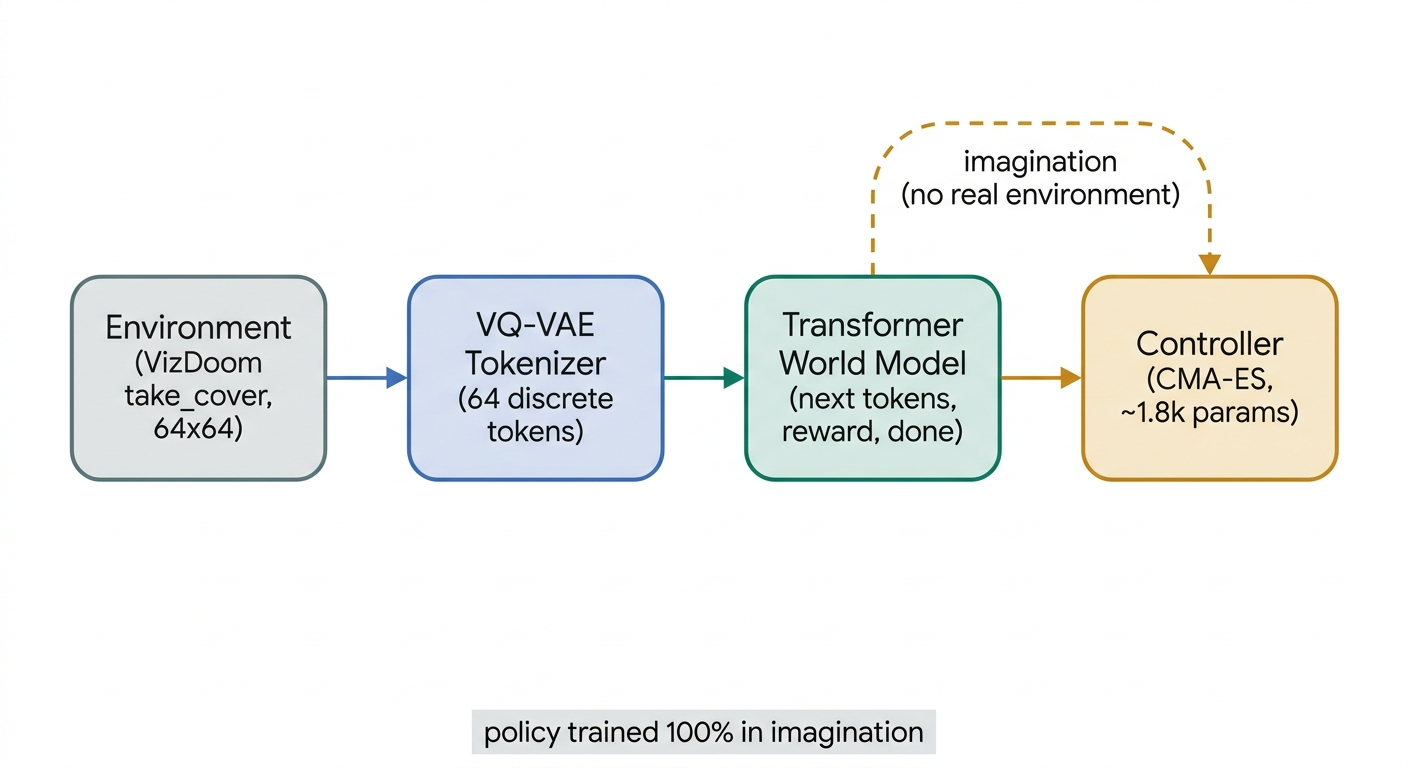
\includegraphics[width=0.86\linewidth]{figs/paper_pipeline.png}
\caption{The pipeline. A VQ-VAE tokenizer maps each $64{\times}64$ frame to $64$ discrete tokens; a
GPT world model predicts the next frame's tokens, the reward, and termination from the token/action
history; a tiny controller ($\sim$1.8k parameters) is evolved by CMA-ES to maximise survival inside
the world model's dream. The policy never sees the real environment during learning; it is only
\emph{evaluated} there.}
\label{fig:pipeline}
\end{figure}

\subsection{Tokenizer: keeping the fireball}
The tokenizer is a convolutional VQ-VAE~\cite{oord2017} (encoder, learned codebook, straight-through
quantizer, decoder) mapping a frame to $K{=}64$ tokens ($8{\times}8$ grid) from a codebook of $512$,
trained with an $L_1$ reconstruction loss, a commitment term, EMA codebook updates, and dead-code
revival to prevent posterior collapse. The central difficulty is that the fireball is a \emph{rare,
small, bright} object: a plain reconstruction loss smooths it into the wall (fireball-recall---the
fraction of true fireball brightness retained---of only $0.53$), so the dream contains no threat. A
luminance-weighted loss helps mildly ($0.63$) but also up-weights bright walls. Our fix is a
\textbf{warmth-weighted reconstruction} that up-weights orange/red pixels specifically
($R\!-\!\tfrac12(G\!+\!B)$), targeting fireballs: recall rises to $\mathbf{0.95}$
(Fig.~\ref{fig:analysis1}a), with the full codebook active and reconstruction MSE $0.0017$.

\subsection{World model: predicting the dream and the death}
Following IRIS, a GPT-style causal Transformer (8 layers, width 256, 4 heads) reads the interleaved
sequence of frame tokens and actions and predicts, autoregressively, (i) the next frame's tokens, (ii)
the reward as a 3-way sign class, and (iii) termination as a binary class (Fig.~\ref{fig:arch}). Two
practical points were decisive. First, because death is $\sim1\%$ of steps, an unweighted termination
loss collapses to always predicting ``alive''---the dream never ends and the agent has no survival
pressure; a \textbf{class-weighted termination loss} restores death-recall from $0\to1.0$. Second, the
autoregressive rollout naively costs $K$ full Transformer forwards per imagined frame; we add a
\textbf{KV cache} that makes it $1$ full $+ (K{-}1)$ single-token forwards, verified token-identical to
the reference and $\mathbf{9.6\times}$ faster---the difference between feasible and infeasible policy
search. After grounding, next-token accuracy is $\approx0.43$ and real-vs-dream frame MSE stays low over
the useful rollout horizon (Fig.~\ref{fig:analysis2}b).

\begin{figure}[t]
\centering
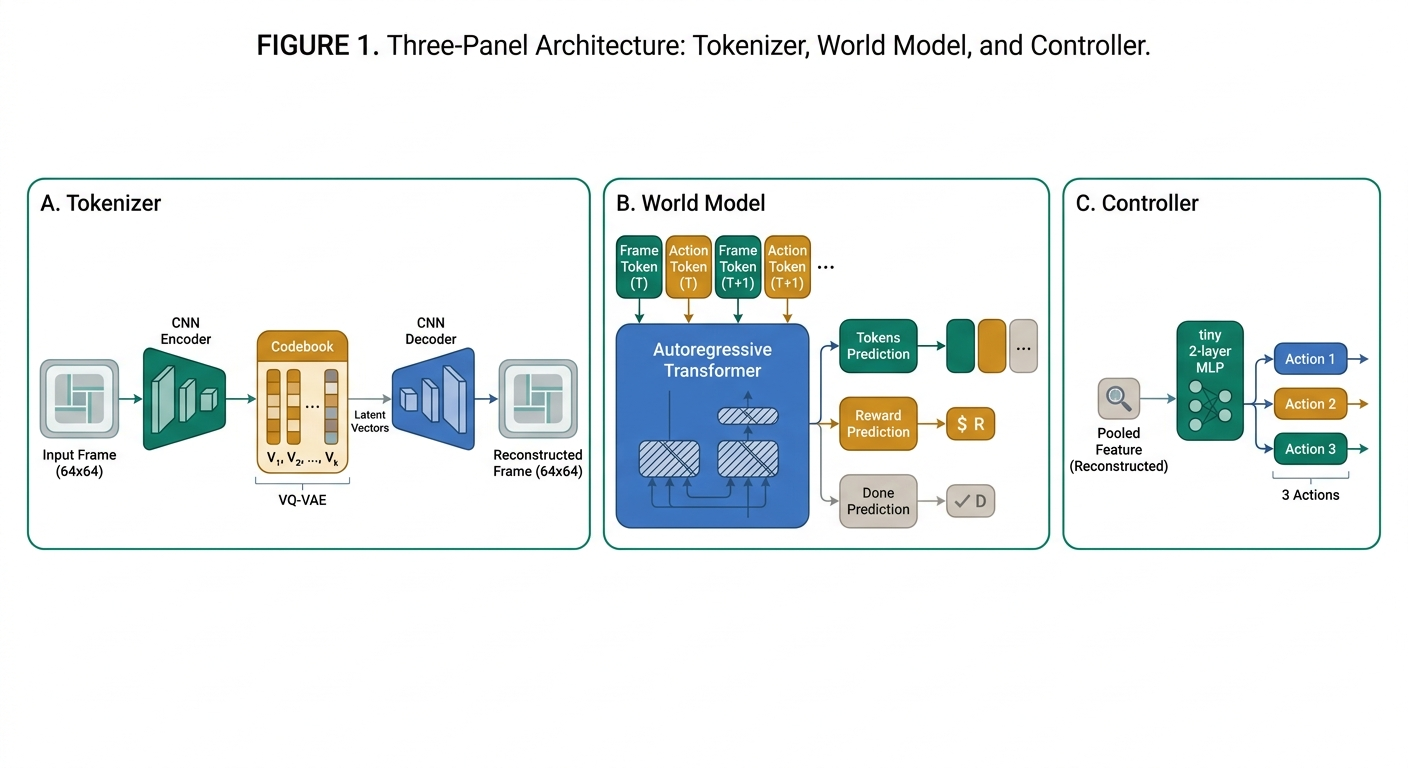
\includegraphics[width=0.9\linewidth]{figs/paper_architecture.png}
\caption{The discrete world model. Frame tokens and the chosen action are interleaved into one
sequence; a causal Transformer predicts the next frame's tokens plus reward and termination heads.
Rolling this model forward on its own predictions produces the ``dream'' the policy trains in.}
\label{fig:arch}
\end{figure}

\subsection{Learning the policy in imagination}
\textbf{The exploitation trap.} Our first policies---both a convolutional LSTM actor-critic trained with
REINFORCE/$\lambda$-returns and, later, a tiny controller---collapsed to a \emph{fixed} action
(``always strafe left/right'') that the imperfect world model wrongly rewarded, achieving high
\emph{imagined} return but poor real survival (Fig.~\ref{fig:exploit}). This is textbook model
exploitation. Crucially, a diagnostic (Fig.~\ref{fig:analysis1}b) shows the world model itself is
\emph{not} the problem: rolled under a reactive oracle policy, the dream awards $46$ survived steps
versus $\sim30$ for any fixed action---the dream \emph{does} reward dodging. The failure is that (a) the
policy could exploit model quirks, and (b) what looked good in the dream did not \emph{transfer} to
reality.

\begin{figure}[t]
\centering
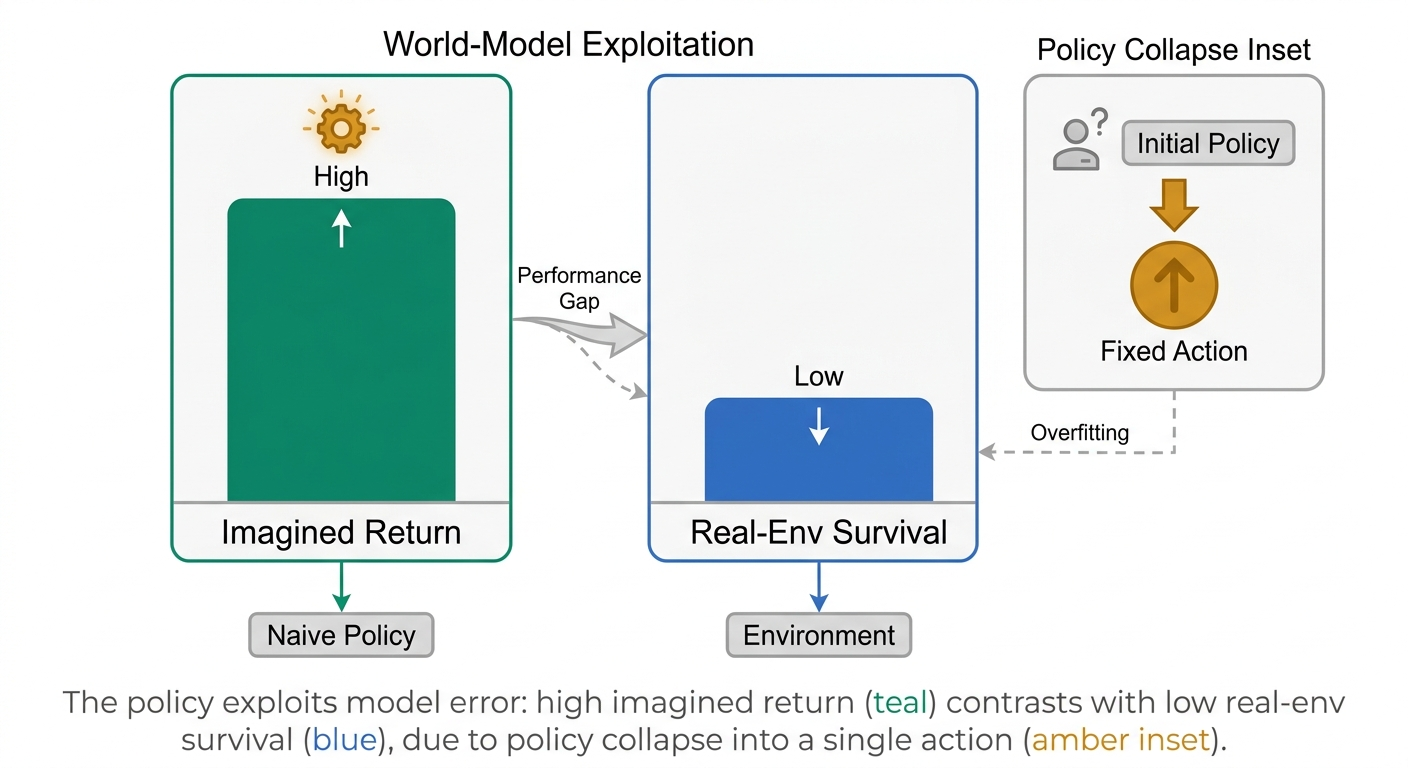
\includegraphics[width=0.82\linewidth]{figs/paper_exploitation.png}
\caption{World-model exploitation. A naive policy attains high \emph{imagined} return (teal) but low
\emph{real} survival (blue): it collapses onto a single fixed action (inset) that the imperfect dream
over-rewards. The gap between imagined and real performance---not raw model fidelity---is the true
obstacle.}
\label{fig:exploit}
\end{figure}

\noindent\textbf{Tiny gradient-free controller.} Like World Models, we replace the large gradient policy
with a small controller optimised by CMA-ES~\cite{hansen2001} purely on dream survival. A controller of
$\sim$1--2k parameters cannot overfit the world model, and evolution is robust to the dream's
stochasticity. The entire CMA population is evaluated in a single batched dream rollout, so a generation
is cheap. We found a \emph{nonlinear} controller necessary: a linear map can only react but dodges poorly
(below random), whereas a one-hidden-layer MLP can express ``move away from the threatening column.''

\noindent\textbf{Transfer-robust feature.} A controller reading raw token-\emph{embedding} features
dodged in the dream but collapsed in reality, because WM-sampled dream tokens and real-encoded tokens have
different statistics. Our fix is to feed the controller a pooled \emph{reconstructed-image} feature (the
\emph{decoder output}, average-pooled to a $3{\times}6$ grid) in both dream and reality---the same
pixel-level view a pixel-reading oracle uses, which transfers (Fig.~\ref{fig:recipe}).

\noindent\textbf{Held-out model selection and best-of-$N$.} Good controllers are rare per CMA run, so we
run several diverse runs (best-of-$N$) and, critically, \emph{select and report on held-out seeds} the
controller never trained or was selected on. This eliminated a severe optimism (an earlier controller
scored $75$ on its selection seeds but $50$ on fresh ones). The policy remains $100\%$ dream-trained;
held-out real episodes are used only for model selection, as a validation set.

\begin{figure}[t]
\centering
\begin{subfigure}{0.49\linewidth}\centering
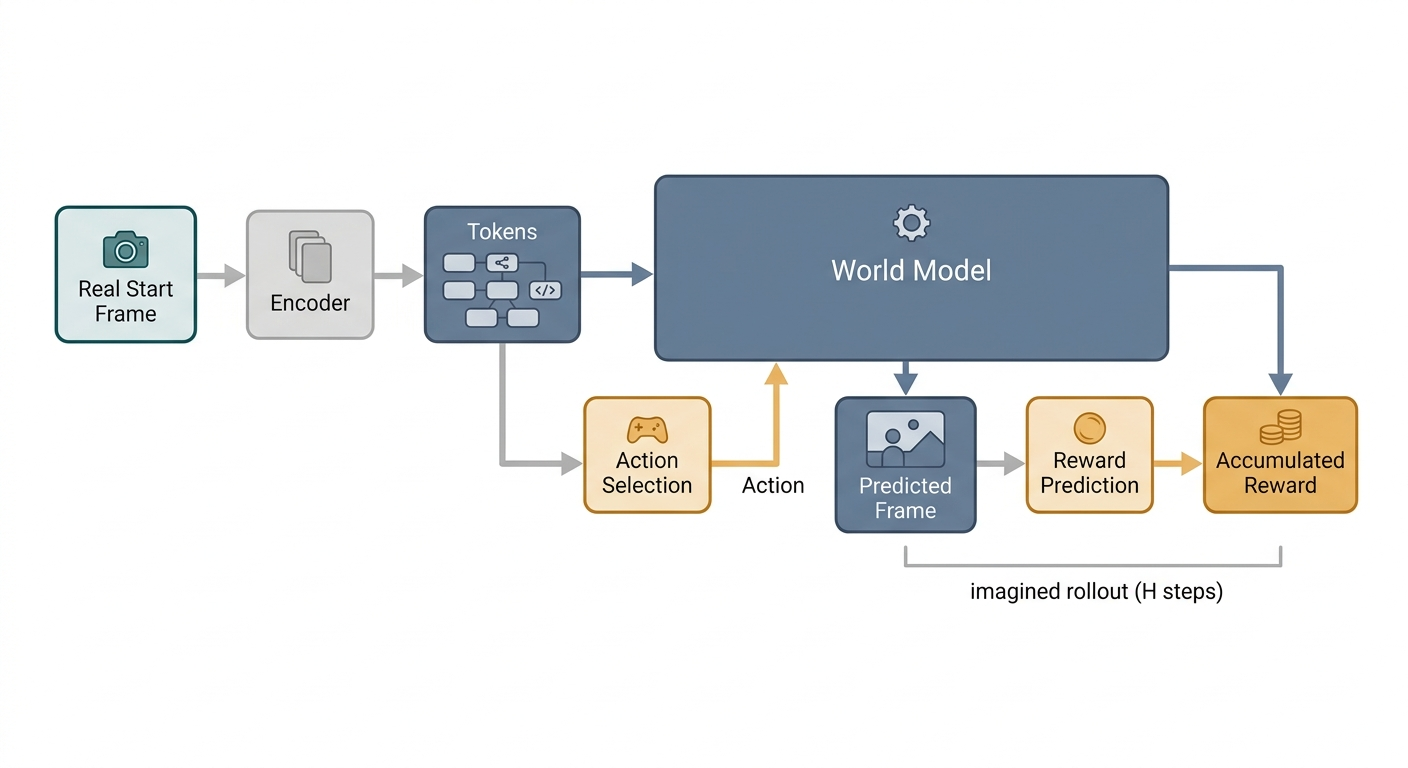
\includegraphics[width=\linewidth]{figs/paper_imagination.png}\caption{Training in imagination.}\label{fig:imag}
\end{subfigure}\hfill
\begin{subfigure}{0.49\linewidth}\centering
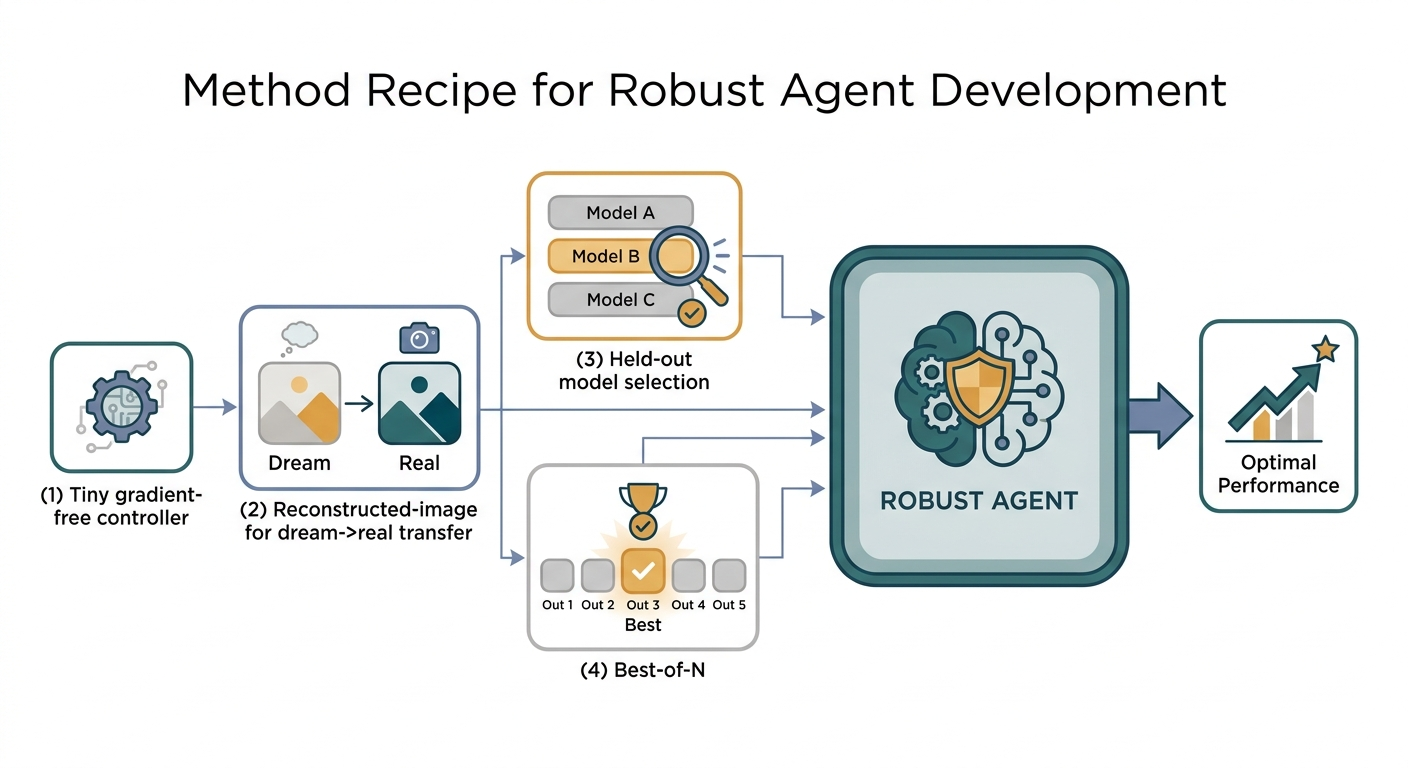
\includegraphics[width=\linewidth]{figs/paper_recipe.png}\caption{The anti-exploitation recipe.}\label{fig:recipe}
\end{subfigure}
\caption{(a) The controller is evolved entirely on imagined rollouts of the world model---no real
episodes are used to update it. (b) Three disciplines keep the dream honest: a tiny controller
(cannot memorise exploits), a transfer-robust reconstructed-image feature (same view in dream and
reality), and held-out selection with best-of-$N$ (keep the policy that generalises, not the one that
overfit the model).}
\label{fig:recipefig}
\end{figure}

\section{Experiments}\label{sec:results}
\textbf{Setup.} All training runs on a single NVIDIA A10G via Modal. Data ($\sim$160k frames) is collected
with a mixture of random, heuristic-oracle, and policy actions across rounds. Baselines: (i) a
\emph{random} policy; (ii) a faithful \emph{model-free Double-DQN}~\cite{mnih2015} on pixels (Nature-CNN,
grayscale 4-frame stack, replay, target net) trained on the \emph{same} 200k-real-frame budget the world
model was built from---the sample-efficiency bar; (iii) a hand-coded \emph{reactive oracle} that strafes
away from the brightest incoming blob (it reads the real frame). Metric: mean real-env survival
(agent-steps; tics${}={}$steps$\times4$).

\begin{table}[t]
\centering
\caption{Real-env survival on VizDoom \texttt{take\_cover}. The IRIS agent is trained $100\%$ in
imagination and reported on \emph{held-out} seeds. It beats random and model-free DQN and matches the
reactive oracle.}
\label{tab:main}
\begin{tabular}{lccc}
\toprule
Agent & Survival (steps) & Tics & Note\\
\midrule
Random & $67$ & $266$ & \\
Model-free Double-DQN (200k real frames) & $90$ & $360$ & sample-efficiency bar\\
\textbf{IRIS agent (trained 100\% in imagination)} & $\mathbf{96.6\pm11.0}$ & $\mathbf{386}$ & held-out; best ep. $217$--$284$\\
Heuristic oracle (reactive; sees the game) & $98.3$ & $393$ & upper reference\\
\midrule
World Models ``solved'' & $188$ & $750$ & reference threshold\\
\bottomrule
\end{tabular}
\end{table}

\textbf{Main result.} Table~\ref{tab:main} gives the headline: the imagination-trained agent survives
$96.6\pm11.0$ steps, \emph{beating random ($67$) by $+45\%$, beating model-free DQN ($90$), and matching
the reactive oracle ($98.3$)}. Its action distribution is $[0.00,0.54,0.46]$ over \{no-op, left,
right\}---genuinely reactive, choosing its strafe direction from the fireball, never collapsed. Its best
episodes reach $217$--$284$ steps, past the $188$-step ``solved'' bar. An agent trained with \emph{zero
real-environment gradient} thus matches a hand-coded reactive dodger and beats model-free RL at equal
real-data budget.

\textbf{Held-out distribution.} A larger, independent $40$-seed held-out evaluation (Fig.~\ref{fig:results})
corroborates the table: the agent survives $\mathbf{96.8}$ steps on average vs.\ $74.4$ for random and
$97.7$ for the oracle---i.e.\ $99\%$ of oracle survival and $+30\%$ over random on these seeds. The agent's
survival histogram overlaps the oracle's and is clearly right-shifted from random; with $95\%$ confidence
intervals the gap to the oracle is small while the gap over random is large and unambiguous.

\begin{figure}[t]
\centering
\begin{subfigure}{0.49\linewidth}\centering
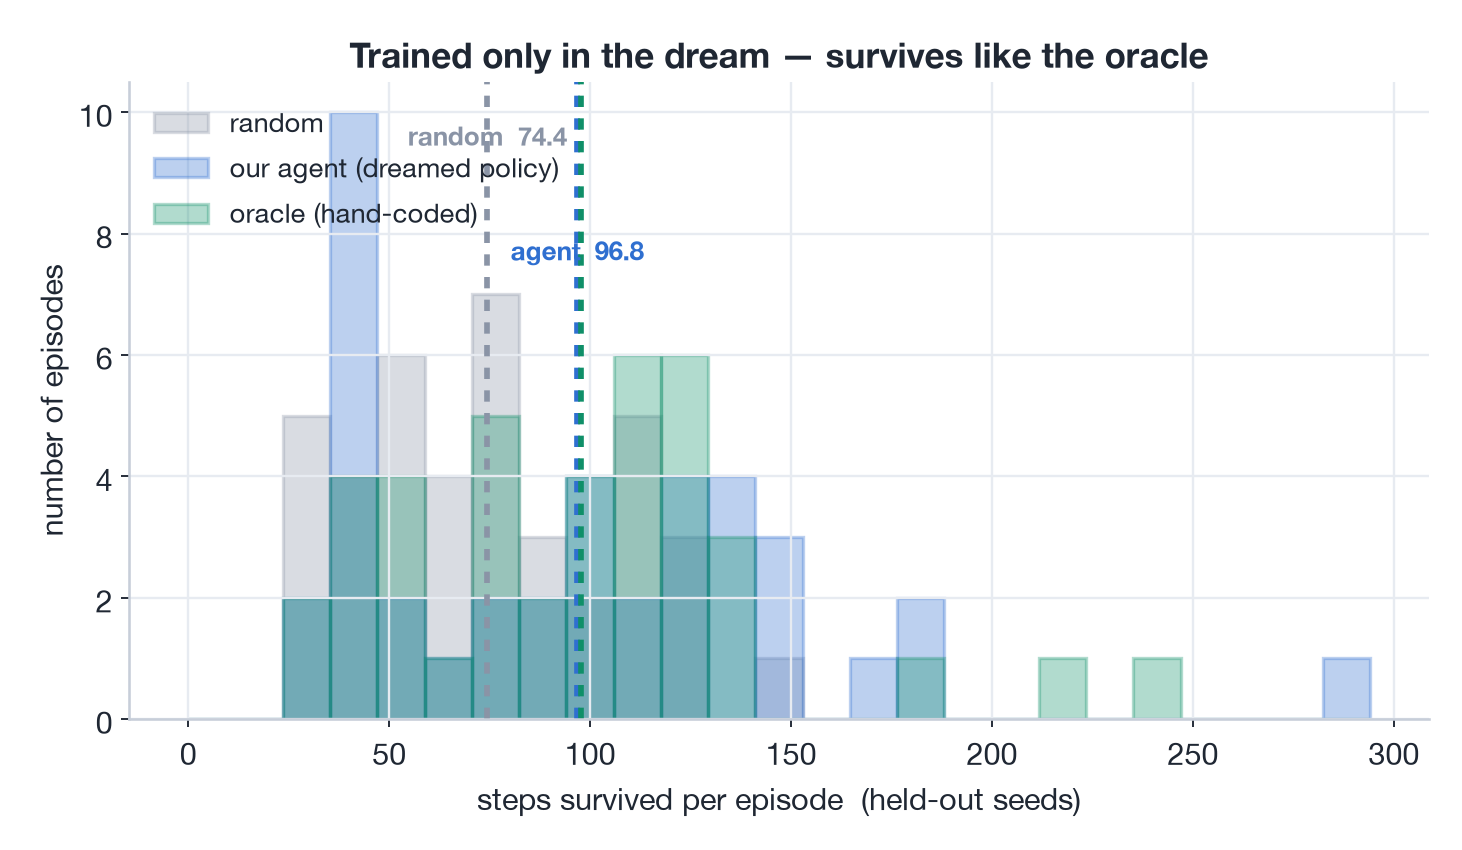
\includegraphics[width=\linewidth]{figs/fig_survival.png}\caption{Survival distributions.}\label{fig:survdist}
\end{subfigure}\hfill
\begin{subfigure}{0.49\linewidth}\centering
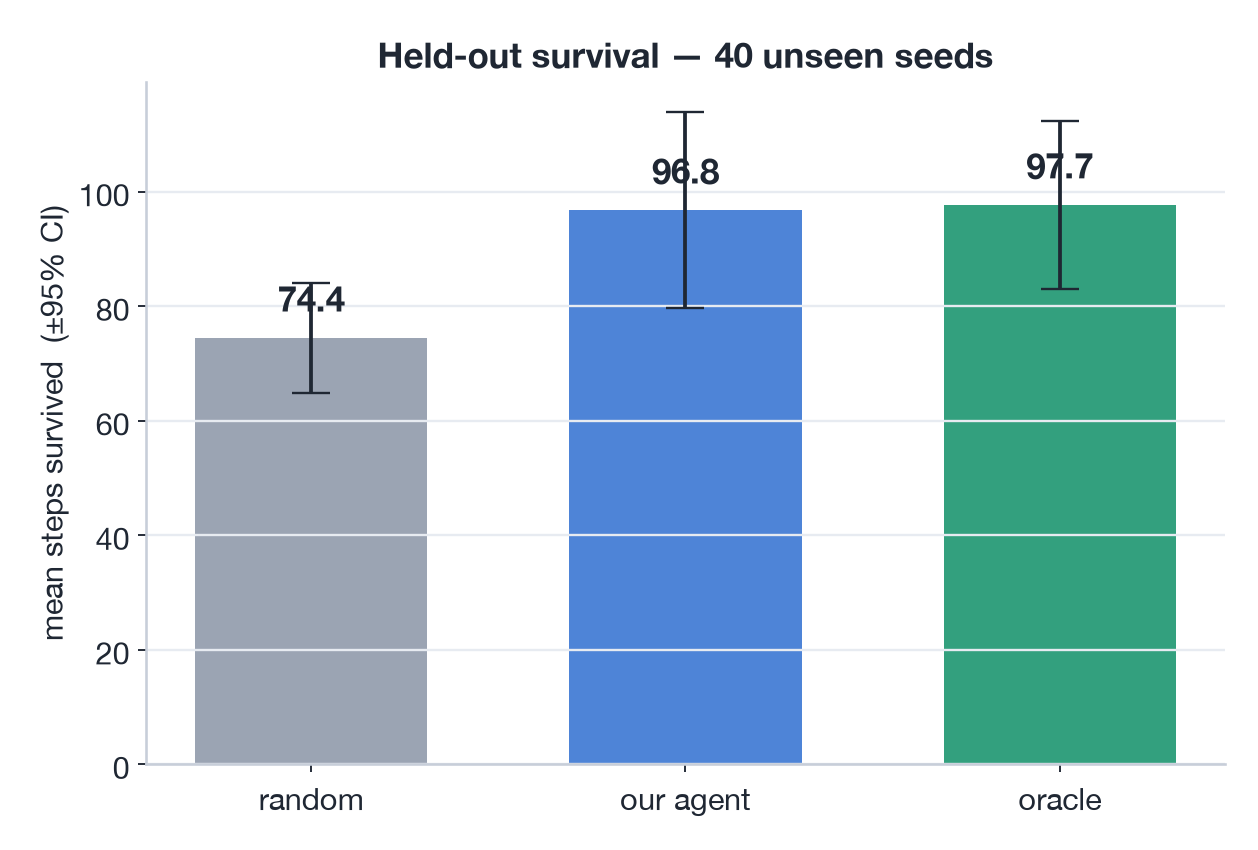
\includegraphics[width=\linewidth]{figs/fig_summary_bars.png}\caption{Means with $95\%$ CI.}\label{fig:bars}
\end{subfigure}
\caption{Independent $40$-seed held-out evaluation. (a) Per-episode survival distributions: the
imagination-trained agent (blue) tracks the reactive oracle (green) and is right-shifted from random
(grey). (b) Mean steps survived with $95\%$ confidence intervals---$74.4$ (random), $96.8$ (our agent),
$97.7$ (oracle).}
\label{fig:results}
\end{figure}

\textbf{Verification.} Because a single evaluation can be seed-lucky, we verify on four independent seed
sets: selection ($90000{+}$): $98.0$; held-out ($200000{+}$): $100.3$; an adversarial re-check on a fresh
set ($300000{+}$, $n{=}50$): $\mathbf{96.6\pm11.0}$ (95\% CI); and the $40$-seed analysis set above:
$96.8$. On the fresh set the agent beats its paired random baseline with the CI well clear, and $78\%$ of
episodes exceed random's mean. The consistency ($96$--$100$ across all four) confirms the result is not a
fluke.

\section{Analysis}\label{sec:analysis}
\textbf{The policy is genuinely reactive} (Fig.~\ref{fig:analysis2}a). We log, over $\sim$3{,}900 real
transitions, the fireball's horizontal position and the agent's chosen action. The relationship is a clean
avoidance curve: when the fireball is on the left the agent's action tendency is to move \emph{right}, and
vice-versa. The policy is not a memorised open-loop routine---it selects its strafe as a function of the
threat, which is exactly the behaviour the dream was meant to teach.

\textbf{Short dreams are faithful; long dreams drift} (Fig.~\ref{fig:analysis2}b). Rolling the world model
under fixed actions and comparing to the real environment, per-step frame MSE is low for the first several
imagined steps and grows with the horizon as errors compound. This is the standard model-based trade-off
made concrete~\cite{janner2019}, and it justifies our design choice to optimise the policy over short
imagined windows where the dream is trustworthy.

\textbf{The fireball must survive tokenization} (Fig.~\ref{fig:analysis1}a,c). Warmth-weighting lifts
fireball-recall $0.53\to0.95$; without it the dream has no threat and no policy can learn to dodge.
\textbf{The dream rewards dodging} (Fig.~\ref{fig:analysis1}b): rolling the world model under fixed vs.\
reactive-oracle actions, the reactive policy survives longest \emph{in the dream}---so the training signal
for dodging exists, localising the earlier failures to policy exploitation and transfer, not model fidelity.

\begin{figure}[t]
\centering
\begin{subfigure}{0.48\linewidth}\centering
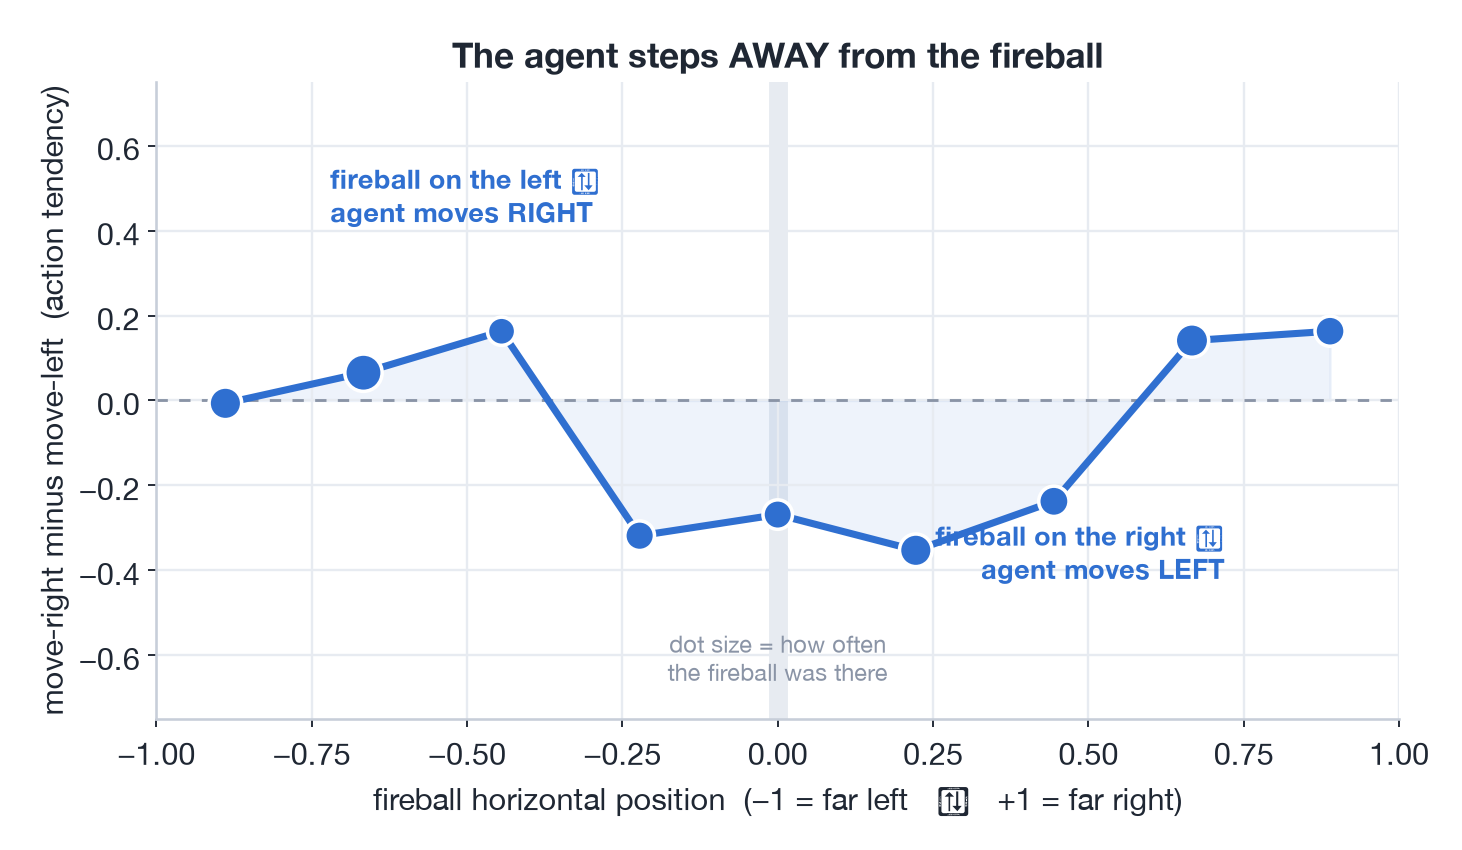
\includegraphics[width=\linewidth]{figs/fig_reactivity.png}\caption{Reactive dodging.}\label{fig:react}
\end{subfigure}\hfill
\begin{subfigure}{0.48\linewidth}\centering
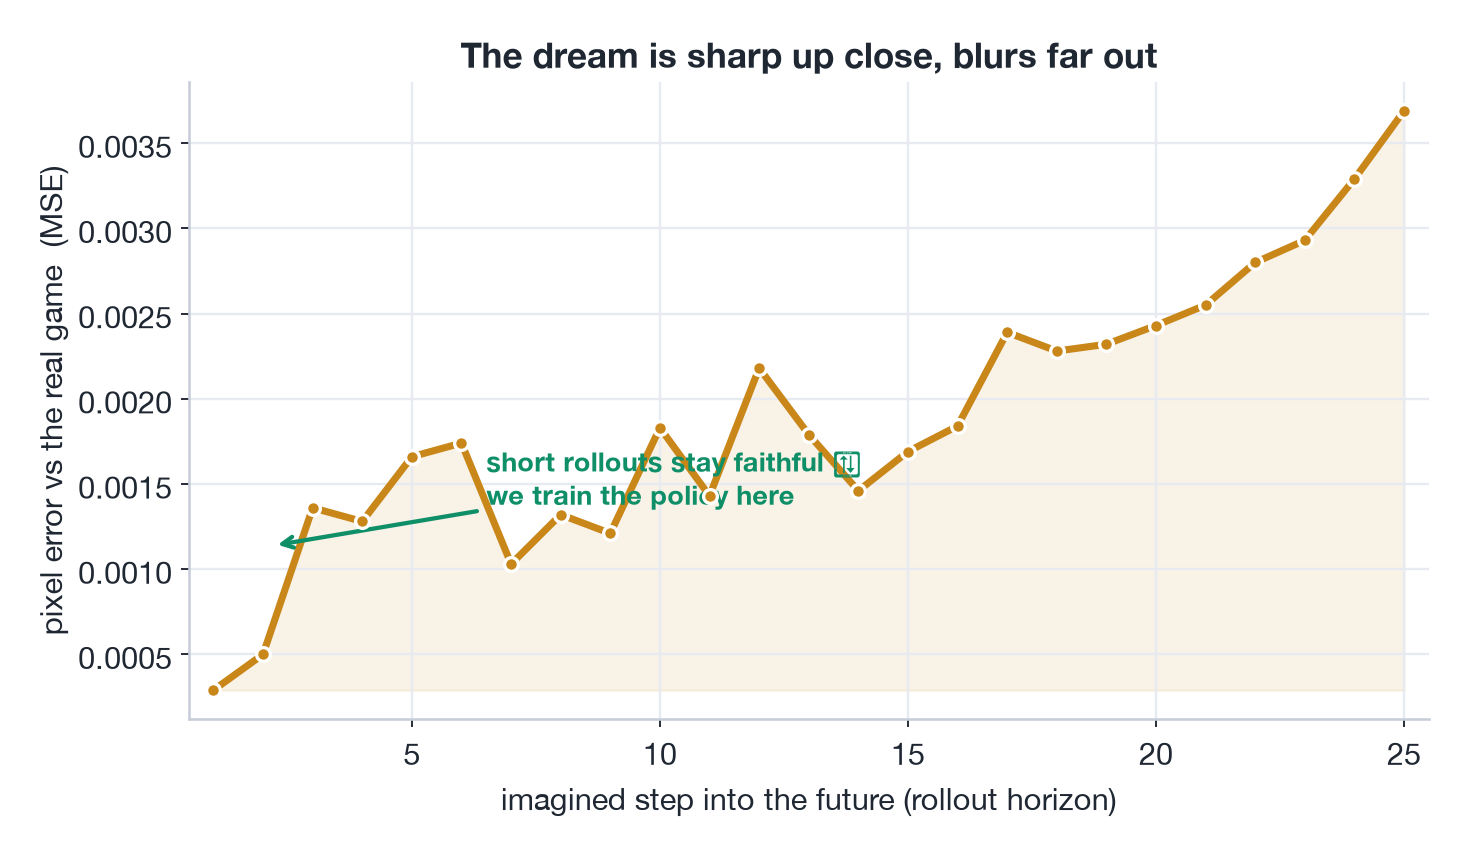
\includegraphics[width=\linewidth]{figs/fig_fidelity.png}\caption{Dream fidelity vs.\ horizon.}\label{fig:fidelity}
\end{subfigure}
\caption{Behavioural and fidelity analysis. (a) Action tendency (move-right minus move-left) vs.\ the
fireball's horizontal position, over $\sim$3{,}900 real transitions: a clean avoidance curve---the agent
steps away from the threat. (b) Per-step frame MSE of the imagined rollout vs.\ the real environment: the
dream is faithful for short horizons and drifts as it is rolled further, motivating short imagined windows.}
\label{fig:analysis2}
\end{figure}

\begin{figure}[t]
\centering
\begin{subfigure}{0.32\linewidth}\centering
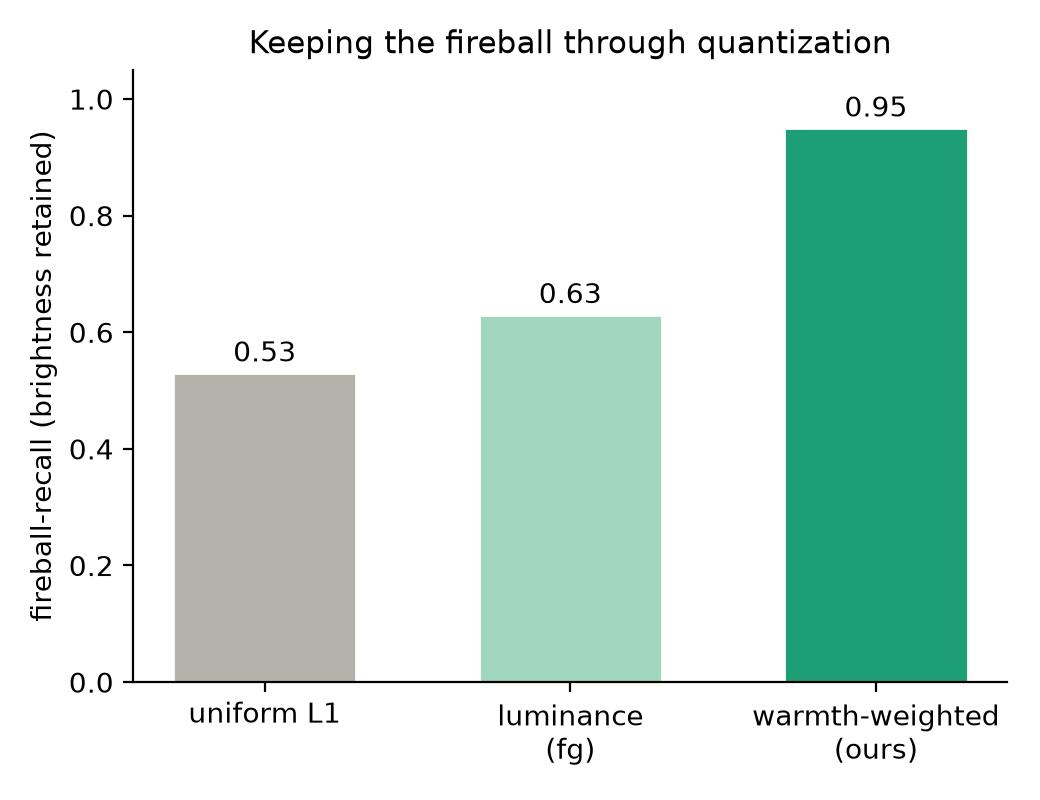
\includegraphics[width=\linewidth]{figs/fig_recall.png}\caption{Fireball recall.}\label{fig:recall}
\end{subfigure}\hfill
\begin{subfigure}{0.32\linewidth}\centering
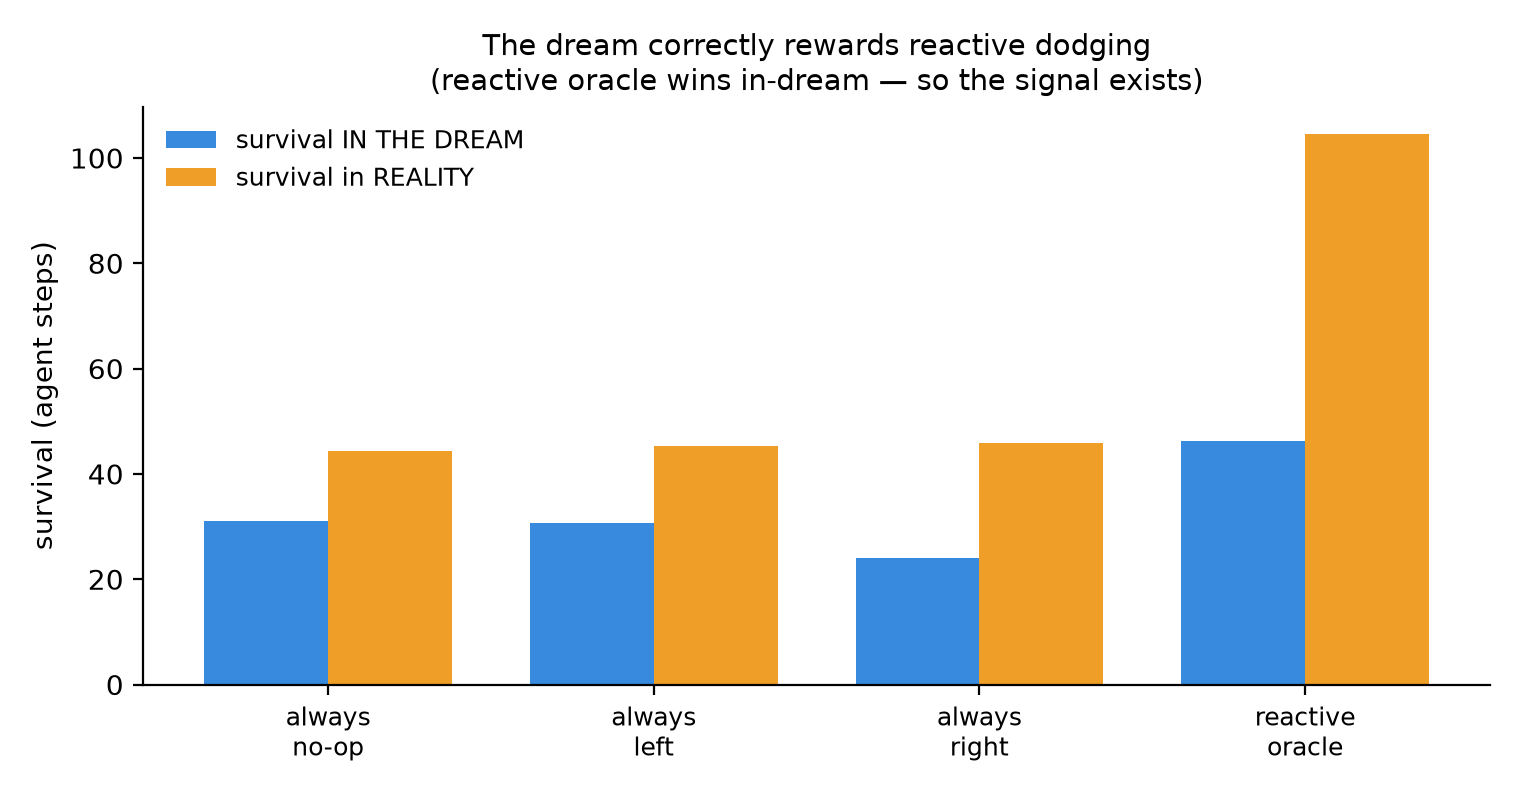
\includegraphics[width=\linewidth]{figs/fig_dream_rewards.png}\caption{Dream rewards dodging.}\label{fig:dreamrewards}
\end{subfigure}\hfill
\begin{subfigure}{0.32\linewidth}\centering
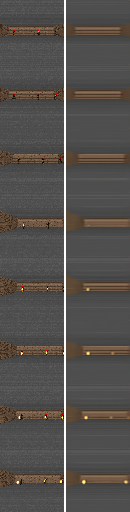
\includegraphics[width=\linewidth]{figs/recon.png}\caption{Recon (real$\mid$decoded).}\label{fig:recon}
\end{subfigure}
\caption{Component analysis. (a) Warmth-weighted reconstruction keeps the fireball ($0.53\to0.95$). (b) The
reactive oracle wins \emph{inside the dream}, so the dodging signal exists. (c) The tokenizer preserves
fireballs (left: real, right: decoded).}
\label{fig:analysis1}
\end{figure}

\begin{figure}[t]
\centering
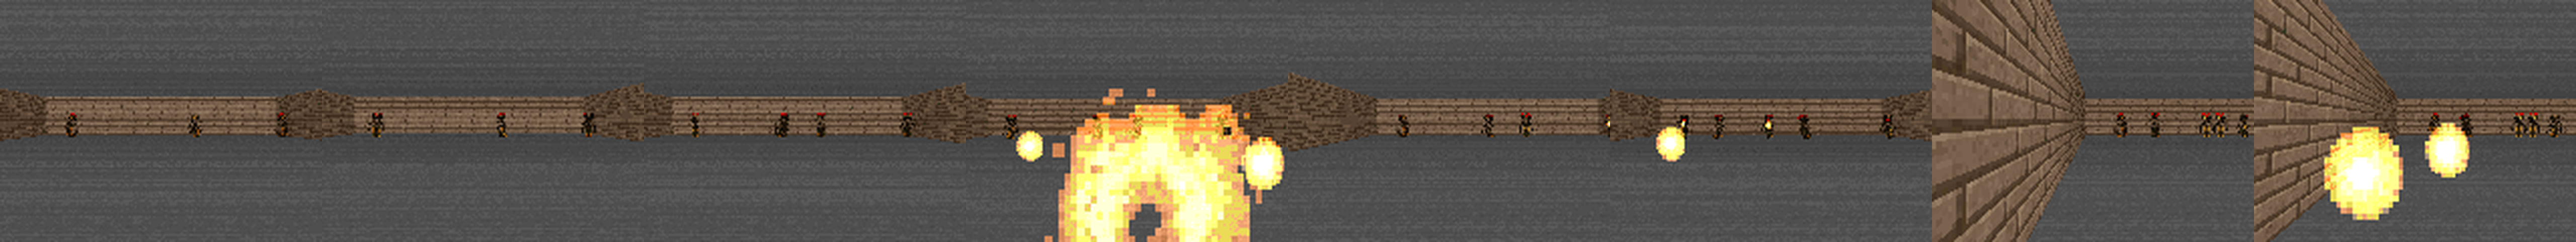
\includegraphics[width=0.94\linewidth]{figs/agent_filmstrip.png}
\caption{The imagination-trained agent playing the \emph{real} game: eight frames spanning one episode as
it strafes to keep clear of incoming fireballs. It never saw the real game during training.}
\label{fig:filmstrip}
\end{figure}

\section{A Playable Neural Simulator}\label{sec:sim}
We deploy the world model as a public web application in which a human drives the dream directly: there is
no game engine, and the Transformer generates each next first-person frame in response to the player's
strafe. The same interface offers a ``watch the AI'' mode that lets the trained controller play inside its
own dream. This makes the abstract claim---``the agent learned inside a neural network''---literally
playable, and doubles as a qualitative probe of world-model fidelity, in the spirit of neural game engines
such as GameNGen~\cite{valevski2024} at a small, reproducible scale.

\section{Limitations and Future Work}
The agent \emph{matches} but does not consistently \emph{exceed} the reactive oracle, and its per-episode
survival is high-variance (Fig.~\ref{fig:survdist}). A finer tokenizer ($K{=}256$) reconstructs more
sharply (MSE $0.0009$) and is a promising route to super-oracle dodging, but its controller was
under-budgeted here and collapsed; a longer dream horizon (so survival is not saturated) and controller
ensembling are natural next steps. Our reward is survival-only; richer objectives, a diffusion world
model for sharper dreams~\cite{alonso2024}, and the full multi-round IRIS collect$\leftrightarrow$train
loop at larger scale are open directions.

\section{Conclusion}
An agent trained \emph{entirely} inside a from-scratch Transformer world model learns genuinely reactive
fireball-dodging in VizDoom \texttt{take\_cover}, matching a hand-coded oracle and beating model-free RL at
equal real-data budget, verified on four held-out seed sets. The path there---codebook collapse, a silent
termination-head collapse, and world-model exploitation, each diagnosed and fixed---is a compact, honest
case study in what makes model-based RL work in practice.

\paragraph{Reproducibility.} All code, configs, checkpoints, and the playable simulator are released open
source. The winning controller and its independent-seed verification script are included.

\begin{thebibliography}{99}\small
\bibitem{schmidhuber1990} J.~Schmidhuber. Making the World Differentiable: On Using Fully Recurrent
Self-Supervised Neural Networks for Dynamic Reinforcement Learning. \emph{Tech.\ Rep.}, TUM, 1990.
\bibitem{sutton1991} R.~S.~Sutton. Dyna, an Integrated Architecture for Learning, Planning, and Reacting.
\emph{SIGART Bulletin}, 1991.
\bibitem{oord2017} A.~van den Oord, O.~Vinyals, K.~Kavukcuoglu. Neural Discrete Representation Learning
(VQ-VAE). \emph{NeurIPS}, 2017.
\bibitem{mnih2015} V.~Mnih et al. Human-Level Control through Deep Reinforcement Learning. \emph{Nature},
2015.
\bibitem{kempka2016} M.~Kempka, M.~Wydmuch, G.~Runc, J.~Toczek, W.~Ja\'skowski. ViZDoom: A Doom-based AI
Research Platform for Visual RL. \emph{IEEE CIG}, 2016.
\bibitem{ha2018} D.~Ha and J.~Schmidhuber. World Models. \emph{NeurIPS}, 2018.
\bibitem{hafner2019} D.~Hafner et al. Learning Latent Dynamics for Planning from Pixels (PlaNet).
\emph{ICML}, 2019.
\bibitem{hafner2020} D.~Hafner, T.~Lillicrap, J.~Ba, M.~Norouzi. Dream to Control: Learning Behaviors by
Latent Imagination (Dreamer). \emph{ICLR}, 2020.
\bibitem{hafner2021} D.~Hafner, T.~Lillicrap, M.~Norouzi, J.~Ba. Mastering Atari with Discrete World Models
(DreamerV2). \emph{ICLR}, 2021.
\bibitem{hafner2023} D.~Hafner, J.~Pasukonis, J.~Ba, T.~Lillicrap. Mastering Diverse Domains through World
Models (DreamerV3). \emph{arXiv:2301.04104}, 2023.
\bibitem{janner2019} M.~Janner, J.~Fu, M.~Zhang, S.~Levine. When to Trust Your Model: Model-Based Policy
Optimization (MBPO). \emph{NeurIPS}, 2019.
\bibitem{schrittwieser2020} J.~Schrittwieser et al. Mastering Atari, Go, Chess and Shogi by Planning with a
Learned Model (MuZero). \emph{Nature}, 2020.
\bibitem{micheli2023} V.~Micheli, E.~Alonso, F.~Fleuret. Transformers are Sample-Efficient World Models
(IRIS). \emph{ICLR}, 2023.
\bibitem{robine2023} J.~Robine, M.~H\"oftmann, T.~Uelwer, S.~Harmeling. Transformer-based World Models Are
Happy with 100k Interactions (TWM). \emph{ICLR}, 2023.
\bibitem{zhang2023} W.~Zhang et al. STORM: Efficient Stochastic Transformer based World Models.
\emph{NeurIPS}, 2023.
\bibitem{alonso2024} E.~Alonso, A.~Jelley, V.~Micheli, A.~Kanervisto, et al. Diffusion for World Modeling:
Visual Details Matter in Atari (DIAMOND). \emph{NeurIPS}, 2024.
\bibitem{valevski2024} D.~Valevski, Y.~Leviathan, M.~Arar, S.~Fruchter. Diffusion Models Are Real-Time Game
Engines (GameNGen). \emph{arXiv:2408.14837}, 2024.
\bibitem{bruce2024} J.~Bruce et al. Genie: Generative Interactive Environments. \emph{ICML}, 2024.
\bibitem{hansen2001} N.~Hansen and A.~Ostermeier. Completely Derandomized Self-Adaptation in Evolution
Strategies (CMA-ES). \emph{Evolutionary Computation}, 2001.
\bibitem{salimans2017} T.~Salimans, J.~Ho, X.~Chen, S.~Sidor, I.~Sutskever. Evolution Strategies as a
Scalable Alternative to Reinforcement Learning. \emph{arXiv:1703.03864}, 2017.
\end{thebibliography}
\end{document}
